\documentclass[journal]{IEEEtran}

% Package to commnet out sections.
\usepackage{comment} 

% Package to make referenzes become ``hyperlinks''
\usepackage{hyperref}

% Package for drawings.
\usepackage{tikz}

% Get the encoding and language right.
\usepackage[utf8]{inputenc}
% \usepackage[ngerman]{babel}

\usepackage{graphicx}                  % This is needed for including figures and graphics
\usepackage{amssymb}
\usepackage{epstopdf}
\DeclareGraphicsRule{.tif}{png}{.png}{`convert #1 `dirname #1`/`basename #1 .tif`.png}

\title{VP Bericht - Elektronik D}
\author{Julian Viereck}
\date{\today}                                           % Activate to display a given date or no date

\begin{document}
\maketitle

\begin{abstract}
\end{abstract}

\tableofcontents

\section{Introduction}

In this experiment, some of the basic concepts of digital circuits are explored.
Digital circuits contain logic gate. The gates transform a
digital input signal into some digital output signal following a well defined functionality.
The input and output signal are either ``high/1'' or ``low/0''. This is a main
difference compared to the analogous circuits, which have a continuous range of
input/output signals. In today's world gates play an important role in. Every
digital circuit contains a few up to multiple billions of them.

Gates can be categorized by gate-family, that they belong to (e.g. TTL or CMOS)
and some other specific properties. Gates perform different operations to
``compute'' the output signal based on some input signal. Also, gates differ in
terms of propagation delay, which is the delay a change in one of the input
signals takes to cause a change in the output signal. The propagation delay is
very important when designing digital circuits.

In the following, the performed experiments are presented. The experiments
describe how to determine the operation performed by a digital circuit and it's
propagation delay, how a pulse generator is build and how to implement a very
simple bit shifter logic.

\section{Experiment simple logic gate}

\subsection{Samples and measurement setup}

The circuit was setup as shown in image <PLACEHOLDER>. Based on the
different input signals at A and B, different values for the output signal C
were measured. As for the ICs, a HCF4001BE and HCF4011BE were used.

To measure the propagation delay, input signal A was connect to a square wave
voltage generator. Input signal B was connected to ground. The IC HCF4001BE
was used for this measurement. The voltage of the generator was set to 2.9V and
the frequency to 1Hz. The input signal A and output signal C was visualized
using a oscilloscope. The oscilloscope's trigger signal was connected to the voltage
generator.

\subsection{Results}

\begin{figure}
\centering
\begin{tabular}{c c | c || c c | c}
  \multicolumn{2}{c}{4011}
  \multicolumn{5}{c}{4001} \\
  A & B & C & A & B & C \\ \hline
  0 & 0 & 1 & 0 & 0 & 1 \\
  0 & 1 & 1 & 0 & 1 & 0 \\
  1 & 0 & 1 & 1 & 0 & 0 \\
  1 & 1 & 0 & 1 & 1 & 0 \\
  
\end{tabular}
\caption{Truth table measuring IC HCF40011BE and HCF4001BE}
\label{tab:truthtable} 
\end{figure}

 \begin{figure*}
  \begin{tikzpicture}
    \node[anchor=south west,inner sep=0] at (0,0)
    {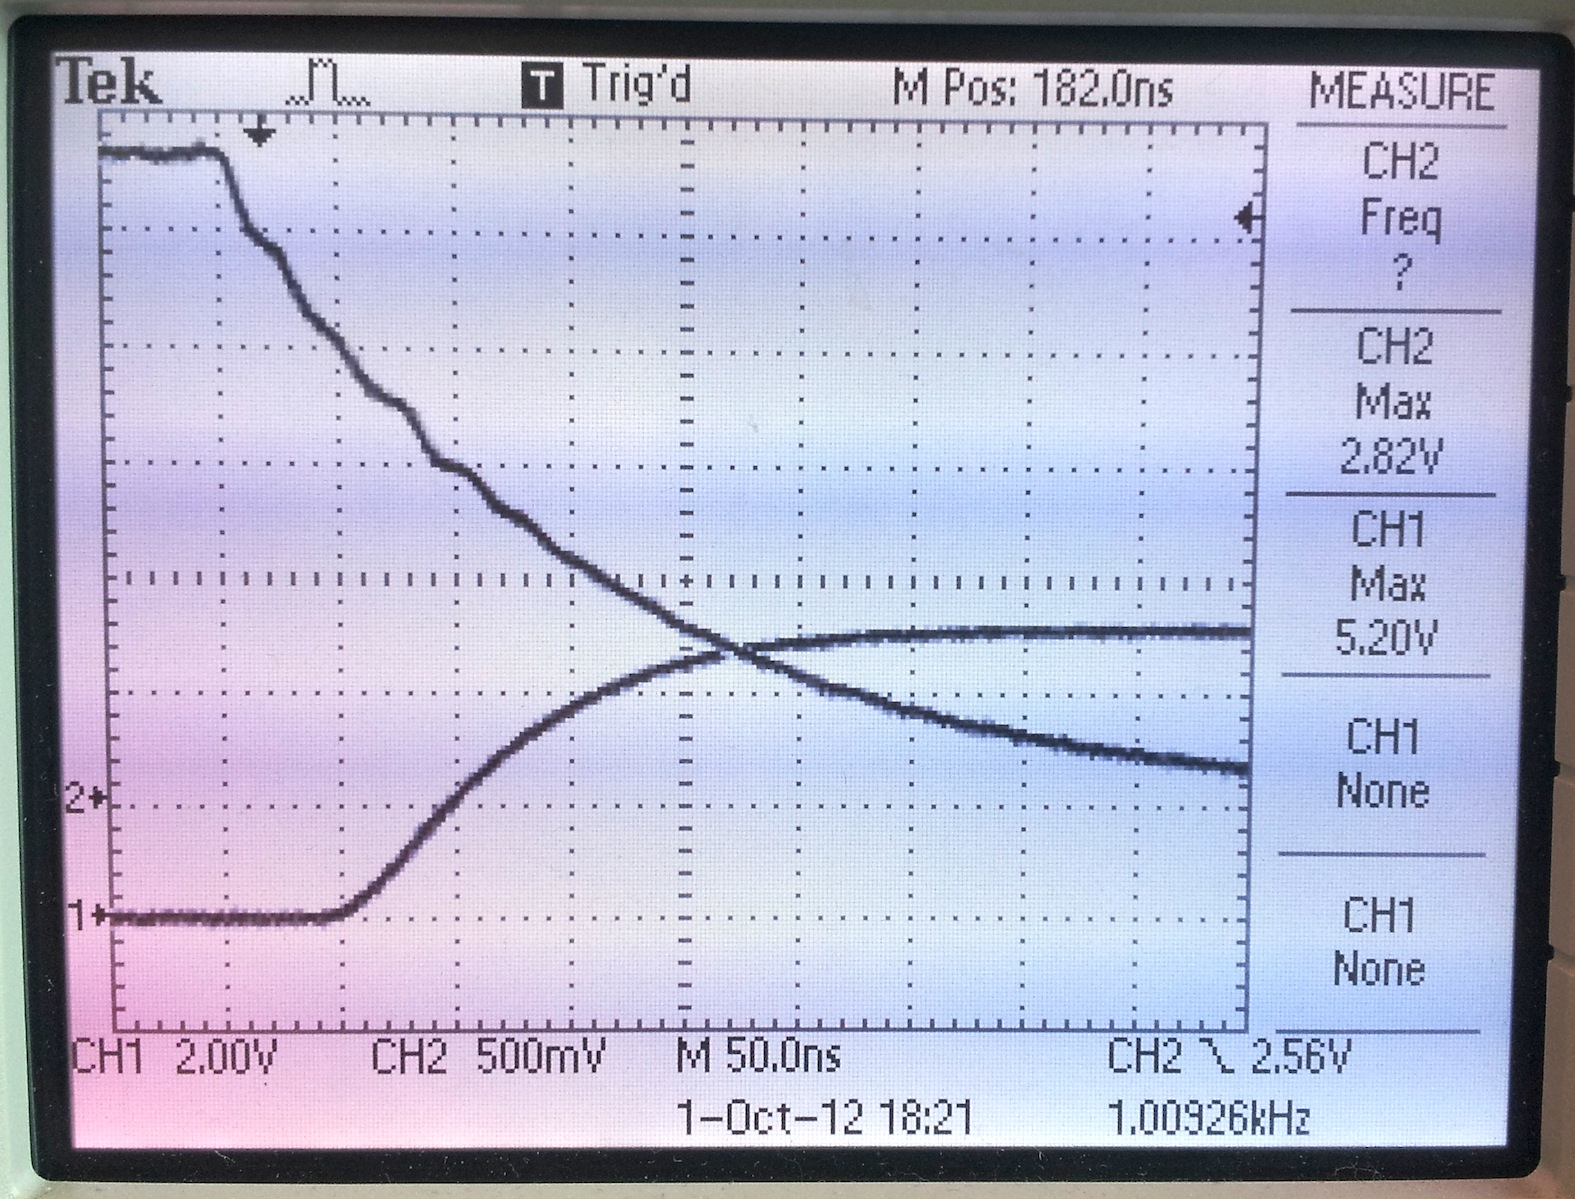
\includegraphics[width=\columnwidth]{img/delay.jpg}};
    \draw[color=red] (1.2,1.1) -- (1.2,6);
    \draw[color=red] (1.9,1.1) -- (1.9,6);
    \path[<->] (1.2, 3) edge node[below]{$\approx 50ns$} (1.9,3);
    \path[<-] (3.3, 3.8) edge node[near end, align=left, right]{Input signal A}
    (4,5);
    \path[<-] (3.3, 2.5) edge node[near end, align=left, right]{Output signal C}
    (4,1.2);
  \end{tikzpicture}
  \caption{Propagation delay measurement.}
  \label{fig:propdelay}
\end{figure*}

For different input signals A and B, the truth-table was measured as
shown in table \ref{tab:truthtable}.

The propagation delay was measured to be around 50ns as seen in figure
\ref{fig:propdelay}.

\subsection{Analysis and Discussion}

Based on the measurements, the IC HCF4001BE seems to be a logic NOR gate,
whereas the IC HCF4011BE seems to function as a NAND gate. This fits with the
specified functionality of the gates.

Looking up the propagation delay from the data sheet, it is said to be typically
around 40ns and up to 75ns. This fits with the here measured delay.

\section{Pulse Generator}

\subsection{Samples and measurement setup}


The circuit was setup as shown in TODO. The period was measured using a
oscilloscope.

\subsection{Functionality explanation}

TODO.

\subsection{Results}

The time diagram for the voltage at point A is shown in \ref{timeA} and for the
point B in \ref{timeB}. In table \ref{ktable} different period times due to
different choices of resistor R and capacitor C are recorded.  

\subsection{Analysis and Discussion}

The k-value is defined by

\begin{equation}
	k = \frac{\Delta t}{R \cdot C}
\end{equation}

where $\Delta t$ is the period time, $R$ is the resistance of the resistor
\em{R} and $C$ is the capacity of the capacitor \em{C}. Based on the
measurements, the k-values are computed in \ref{ktable}.

\subsubsection{Die Analyse der Daten}

\subsubsection{Genauigkeit der bestimmten Parameter}

\subsubsection{Vergleich mit Literaturwerten}

\subsection{Schlussfolgerung und Ausblick }

\section{Die Messmethode und der experimentelle Aufbau}

\section{Die Messergebnisse}

\end{document}
